%%%%%%%%%%%%%%%%%%%%%%%%%%%%% Define Article %%%%%%%%%%%%%%%%%%%%%%%%%%%%%%%%%%
\documentclass{article}
%%%%%%%%%%%%%%%%%%%%%%%%%%%%%%%%%%%%%%%%%%%%%%%%%%%%%%%%%%%%%%%%%%%%%%%%%%%%%%%

%%%%%%%%%%%%%%%%%%%%%%%%%%%%% Using Packages %%%%%%%%%%%%%%%%%%%%%%%%%%%%%%%%%%
\usepackage{geometry}
\usepackage{graphicx}
\usepackage{amssymb}
\usepackage{amsmath}
\usepackage{amsthm}
\usepackage{empheq}
\usepackage{mdframed}
\usepackage{booktabs}
\usepackage{lipsum}
\usepackage{graphicx}
\usepackage{color}
\usepackage{psfrag}
\usepackage{pgfplots}
\usepackage{bm}
\usepackage{enumitem}
\usepackage{subcaption}
\usepackage{multirow}
\usepackage{tabularx}

%%%%%%%%%%%%%%%%%%%%%%%%%%%%%%%%%%%%%%%%%%%%%%%%%%%%%%%%%%%%%%%%%%%%%%%%%%%%%%%

% Other Settings

%%%%%%%%%%%%%%%%%%%%%%%%%% Page Setting %%%%%%%%%%%%%%%%%%%%%%%%%%%%%%%%%%%%%%%
\geometry{a4paper}

%%%%%%%%%%%%%%%%%%%%%%%%%% Define some useful colors %%%%%%%%%%%%%%%%%%%%%%%%%%
\definecolor{ocre}{RGB}{243,102,25}
\definecolor{mygray}{RGB}{243,243,244}
\definecolor{deepGreen}{RGB}{26,111,0}
\definecolor{shallowGreen}{RGB}{235,255,255}
\definecolor{deepBlue}{RGB}{61,124,222}
\definecolor{shallowBlue}{RGB}{235,249,255}
%%%%%%%%%%%%%%%%%%%%%%%%%%%%%%%%%%%%%%%%%%%%%%%%%%%%%%%%%%%%%%%%%%%%%%%%%%%%%%%

%%%%%%%%%%%%%%%%%%%%%%%%%% Define an orangebox command %%%%%%%%%%%%%%%%%%%%%%%%
\newcommand\orangebox[1]{\fcolorbox{ocre}{mygray}{\hspace{1em}#1\hspace{1em}}}
%%%%%%%%%%%%%%%%%%%%%%%%%%%%%%%%%%%%%%%%%%%%%%%%%%%%%%%%%%%%%%%%%%%%%%%%%%%%%%%

%%%%%%%%%%%%%%%%%%%%%%%%%%%% English Environments %%%%%%%%%%%%%%%%%%%%%%%%%%%%%
\newtheoremstyle{mytheoremstyle}{3pt}{3pt}{\normalfont}{0cm}{\rmfamily\bfseries}{}{1em}{{\color{black}\thmname{#1}~\thmnumber{#2}}\thmnote{\,--\,#3}}
\newtheoremstyle{myproblemstyle}{3pt}{3pt}{\normalfont}{0cm}{\rmfamily\bfseries}{}{1em}{{\color{black}\thmname{#1}~\thmnumber{#2}}\thmnote{\,--\,#3}}
\theoremstyle{mytheoremstyle}
\newmdtheoremenv[linewidth=1pt,backgroundcolor=shallowGreen,linecolor=deepGreen,leftmargin=0pt,innerleftmargin=20pt,innerrightmargin=20pt,]{theorem}{Theorem}[section]
\theoremstyle{mytheoremstyle}
\newmdtheoremenv[linewidth=1pt,backgroundcolor=shallowBlue,linecolor=deepBlue,leftmargin=0pt,innerleftmargin=20pt,innerrightmargin=20pt,]{definition}{Definition}[section]
\theoremstyle{myproblemstyle}
\newmdtheoremenv[linecolor=black,leftmargin=0pt,innerleftmargin=10pt,innerrightmargin=10pt,]{problem}{Problem}[section]
%%%%%%%%%%%%%%%%%%%%%%%%%%%%%%%%%%%%%%%%%%%%%%%%%%%%%%%%%%%%%%%%%%%%%%%%%%%%%%%

%%%%%%%%%%%%%%%%%%%%%%%%%%%%%%% Plotting Settings %%%%%%%%%%%%%%%%%%%%%%%%%%%%%
\usepgfplotslibrary{colorbrewer}
\pgfplotsset{width=8cm,compat=1.9}
%%%%%%%%%%%%%%%%%%%%%%%%%%%%%%%%%%%%%%%%%%%%%%%%%%%%%%%%%%%%%%%%%%%%%%%%%%%%%%%

%%%%%%%%%%%%%%%%%%%%%%%%%%%%%%% Title & Author %%%%%%%%%%%%%%%%%%%%%%%%%%%%%%%%
\title{Tarea 2}
\author{Leonel Guerrero 18-10638}
%%%%%%%%%%%%%%%%%%%%%%%%%%%%%%%%%%%%%%%%%%%%%%%%%%%%%%%%%%%%%%%%%%%%%%%%%%%%%%%

\begin{document}
\maketitle
\section{Pregunta 1}

Suponga que tiene el siguiente conjunto de datos en dos dimensiones (x1, x2) con respuesta deseada y:

\begin{table}[h]
  \centering
  \begin{tabular}{ccc}
    \hline
    x1 & x2 & y \\ \hline
    0  & 0  & 0 \\
    1  & 1  & 1 \\
    1  & -1 & 1 \\
    -1 & 0  & 1 \\ \hline
  \end{tabular}
\end{table}

\begin{enumerate}[label=(\alph*)]
  \item Demuestre que el conjunto se podrá clasificar usando el perceptrón de Rosenblatt indicando los pesos sinápticos que harán el trabajo, o en su defecto demuestre matemáticamente que el conjunto no puede clasificarse usando el perceptrón de Rosenblatt

        \textit{Solución:} Primero realicemos una gráfica de los datos para tener un primera aproximación y visualizar la distribución de los datos

        \begin{center}
          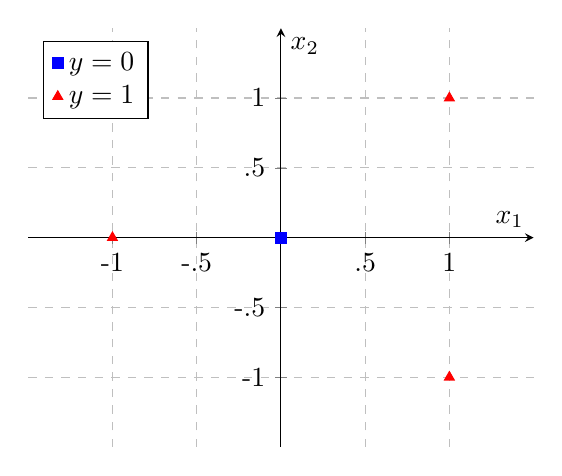
\begin{tikzpicture}
            \begin{axis}[
                scatter/classes={
                    a={mark=square*,blue},
                    b={mark=triangle*,red}
                  },
                xtick={-1,-0.5,0,0.5,1},
                ytick={-1,-0.5,0,0.5,1},
                axis lines=middle,
                xlabel=$x_1$,
                ylabel=$x_2$,
                xmin=-1.5,
                xmax=1.5,
                ymin=-1.5,
                ymax=1.5,
                xticklabels={-1,-.5,0,.5,1},
                yticklabels={-1,-.5,0,.5,1},
                grid=major,
                grid style=dashed,
                legend pos=north west,
              ]
              \addplot[scatter,only marks, scatter src=explicit symbolic] coordinates {
                  (0,0) [a]
                  (1,1) [b]
                  (1,-1) [b]
                  (-1,0) [b]
                };
              \legend{$y=0$,$y=1$}
            \end{axis}
          \end{tikzpicture}
        \end{center}

        Se demostrara que el conjunto no puede clasificarse usando el perceptrón de Rosenblatt. Para poder aplicar el algoritmo del perceptrón de Rosenblatt, se debe cumplir que los datos sean linealmente separables, es decir, que exista una recta que divida los datos en dos conjuntos, uno para cada clase. En este caso, no existe tal recta, por lo que no se puede aplicar el algoritmo del perceptrón de Rosenblatt. Si analizamos la siguiente gráfica

        \begin{center}
          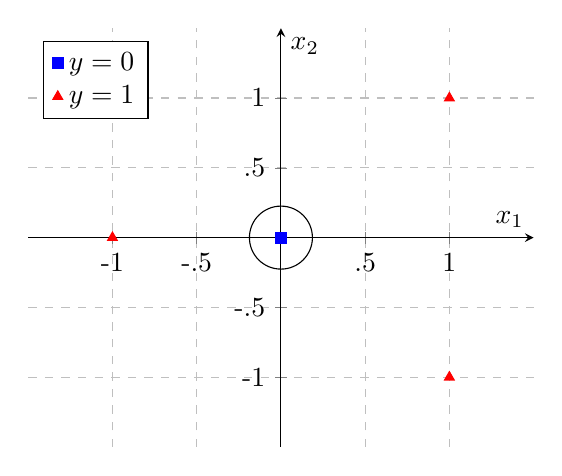
\begin{tikzpicture}
            \begin{axis}[
                scatter/classes={
                    a={mark=square*,blue},
                    b={mark=triangle*,red}
                  },
                xtick={-1,-0.5,0,0.5,1},
                ytick={-1,-0.5,0,0.5,1},
                axis lines=middle,
                xlabel=$x_1$,
                ylabel=$x_2$,
                xmin=-1.5,
                xmax=1.5,
                ymin=-1.5,
                ymax=1.5,
                xticklabels={-1,-.5,0,.5,1},
                yticklabels={-1,-.5,0,.5,1},
                grid=major,
                grid style=dashed,
                legend pos=north west,
              ]
              \addplot[scatter,only marks, scatter src=explicit symbolic] coordinates {
                  (0,0) [a]
                  (1,1) [b]
                  (1,-1) [b]
                  (-1,0) [b]
                };
              \draw (axis cs:0,0) circle [radius=0.4cm];
              \legend{$y=0$,$y=1$}
            \end{axis}
          \end{tikzpicture}
        \end{center}

        Podemos apreciar que ninguna recta tangente a la circunferencia puede dividir los datos en dos conjuntos, por lo que no se puede aplicar el algoritmo del perceptrón de Rosenblatt, ya que no existe una recta que divida los datos en dos conjuntos, uno para cada clase.

  \item Suponga que el conjunto de datos se le agrega una tercera característica $x_3$, tal que $x_3=x^2_1+x^2_2$. Si entrenamos el perceptrón usando el algoritmo primal de de Rosenblatt, ¿podemos garantizar su convergencia? Si el perceptrón clasifica correctamente, explique su razonamiento e indique un conjunto de pesos que definan el plano separador. Si el perceptrón no clasifica correctamente este conjunto, explique la razón y demuéstralo matemáticamente.

        Veamos el conjunto en una tabla

        \begin{table}[h]
          \centering
          \begin{tabular}{cccc}
            \hline
            $x_1$ & $x_2$ & $x_3$ & $y$ \\ \hline
            0     & 0     & 0     & 0   \\
            1     & 1     & 2     & 1   \\
            1     & -1    & 2     & 1   \\
            -1    & 0     & 1     & 1   \\ \hline
          \end{tabular}
        \end{table}

        Ahora analizamos el conjunto de datos, para ver si es linealmente separable. Para esto, graficamos los datos en un espacio tridimensional

        \begin{tabular}{cc}
          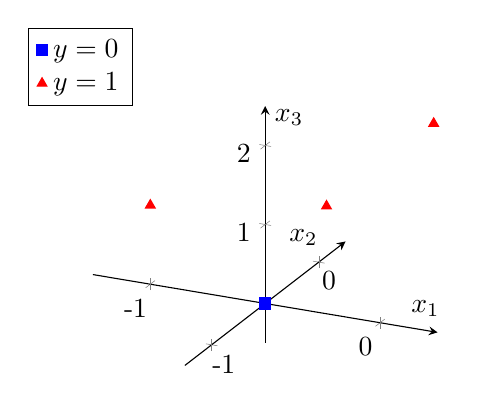
\begin{tikzpicture}
            \begin{axis}[
                scatter/classes={
                    a={mark=square*,blue},
                    b={mark=triangle*,red}
                  },
                xtick={-1,0,1},
                ytick={-1,0,1},
                ztick={0,1,2},
                axis lines=middle,
                xlabel=$x_1$,
                ylabel=$x_2$,
                zlabel=$x_3$,
                xmin=-1.5,
                xmax=1.5,
                ymin=-1.5,
                ymax=1.5,
                zmin=-0.5,
                zmax=2.5,
                xticklabels={-1,-.5,0,.5,1},
                yticklabels={-1,-.5,0,.5,1},
                zticklabels={0,1,2},
                grid=major,
                grid style=dashed,
                legend pos=north west,
              ]
              \addplot3[scatter,only marks, scatter src=explicit symbolic] coordinates {
                  (0,0,0) [a]
                  (1,1,2) [b]
                  (1,-1,2) [b]
                  (-1,0,1) [b]
                };
              \legend{$y=0$,$y=1$}
            \end{axis}
          \end{tikzpicture}
           &
          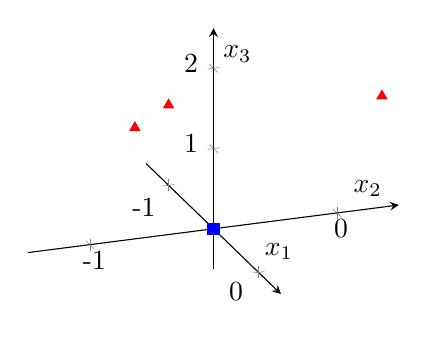
\begin{tikzpicture}
            \begin{axis} [
                scatter/classes={
                    a={mark=square*,blue},
                    b={mark=triangle*,red}
                  },
                xtick={-1,0,1},
                ytick={-1,0,1},
                ztick={0,1,2},
                axis lines=middle,
                xlabel=$x_1$,
                ylabel=$x_2$,
                zlabel=$x_3$,
                xmin=-1.5,
                xmax=1.5,
                ymin=-1.5,
                ymax=1.5,
                zmin=-0.5,
                zmax=2.5,
                xticklabels={-1,-.5,0,.5,1},
                yticklabels={-1,-.5,0,.5,1},
                zticklabels={0,1,2},
                grid=major,
                grid style=dashed,
                view={70}{30},
              ]
              \addplot3[scatter,only marks, scatter src=explicit symbolic] coordinates {
                  (0,0,0) [a]
                  (1,1,2) [b]
                  (1,-1,2) [b]
                  (-1,0,1) [b]
                };
            \end{axis}
          \end{tikzpicture} \\
        \end{tabular}


        Podemos apreciar que el conjunto de datos es linealmente separable, ya que  existe un plano que divida los datos en dos conjuntos, uno para cada clase. Por lo tanto, se podría aplicar el algoritmo del perceptrón de Rosenblatt. Sin embargo se puede apreciar que el plano que divide los datos puede deducirse por medio de la gráfica, ya que podemos calcular el plano deseado partiendo del plano que pasa por los 3 puntos con $y=1$ (rojos), el cual es $x+0y-2z=-3$, y bajarlo para que no pase por los puntos, obteniendo $x+0y-2z=-1.5$

        Podemos apreciarlo de mejor manera por medio de la siguiente graficamos

        \begin{center}

          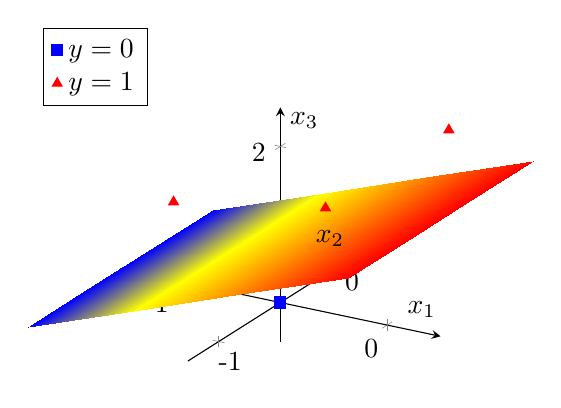
\begin{tikzpicture}
            \begin{axis}[
                scatter/classes={
                    a={mark=square*,blue},
                    b={mark=triangle*,red}
                  },
                xtick={-1,0,1},
                ytick={-1,0,1},
                ztick={0,1,2},
                axis lines=middle,
                xlabel=$x_1$,
                ylabel=$x_2$,
                zlabel=$x_3$,
                xmin=-1.5,
                xmax=1.5,
                ymin=-1.5,
                ymax=1.5,
                zmin=-0.5,
                zmax=2.5,
                xticklabels={-1,-.5,0,.5,1},
                yticklabels={-1,-.5,0,.5,1},
                zticklabels={0,1,2},
                grid=major,
                grid style=dashed,
                legend pos=north west,
                view={30}{30},
              ]
              \addplot3[scatter,only marks, scatter src=explicit symbolic] coordinates {
                  (0,0,0) [a]
                  (1,1,2) [b]
                  (1,-1,2) [b]
                  (-1,0,1) [b]
                };
              \addplot3[surf, domain=-1.5:1.5, samples=4, shader=interp] {(3/4)+(x/2)};
              \legend{$y=0$,$y=1$}
            \end{axis}
          \end{tikzpicture}
        \end{center}

        En donde se puede apreciar que el plano $x+0y-2z=-1.5$ divide los datos en dos conjuntos, uno para cada clase.

\end{enumerate}

\section{Pregunta 2 - Implementación del algoritmo}
Implemente el perceptrón de Rosenblatt para multiples clases en el lenguaje de su preferencia. Deberá entregar el código de este algoritmo con una documentación mínima.

La implementación del algoritmo la podrá encontrar en dos modalidades, un repositorio de GitHub y un link a un notebook de Google Colab.

\begin{itemize}
  \item GitHub:
  \item Google Colab:
\end{itemize}


\section{Pregunta 3 - Resultados}

\subsection{Enunciado}

\begin{table}[h]
  \centering
  \begin{tabular}{ll}
    \hline
    \textbf{Categoría}                 & \textbf{Archivo} \\
    \hline
    Agricultura                        & Agri.csv         \\
    Matemáticas                        & Math.csv         \\
    Ciencias médicas                   & MedSci.csv       \\
    Astrofísica y Astronomía           & AstroAstr.csv    \\
    Química                            & Chem.csv         \\
    Ciencias de la tierra y el espacio & EarthSpace.csv   \\
    Ciencias de la vida                & LifeSci.csv      \\
    Física                             & Physics.csv      \\
    Ciencias Tecnológicas              & TechSci.csv      \\
    \hline
  \end{tabular}
\end{table}

Los archivos en la carpeta de datos contienen representaciones vectoriales de tamaño 512 de textos científicos utilizando el Universal Sentence Encoder. Cada fila en los archivos corresponde a un texto (estímulo) dentro de la categoría que representa el archivo. Se tiene un archivo para 9 categorías:

Entrene la máquina de Rosenblatt (pregunta 2) para la clasificación binaria con el conjunto que corresponde a Ciencias de la tierra y el espacio vs Ciencias médicas.

Entrene el perceptrón inicializando los pesos en el intervalo $[-0.05, 0.05]$ y por 100 épocas usando los valores de $\eta = 0.001,$ $0.01$, y $0.1$. En cada caso indique el porcentaje de acierto al finalizar el entrenamiento y cualquier dificultad en el entrenamiento. Repita el ejercicio ahora para clasificar entre Ciencias de la vida y Agricultura.

\subsection{Presentación de resultados}

A continuación presentaremos el resumen de los resultados en una tabla donde se podrá apreciar el porcentaje de acierto para cada uno de los casos y para cada tasa de aprendizaje, así como la dificultad que se presentó en cada caso.

\begin{table}[h]
  \centering
  \begin{tabular}{cccll}
    \cline{1-4}
    Categorías                                  & \begin{tabular}[c]{@{}c@{}}Tasa de\\ aprendizaje\end{tabular} & \begin{tabular}[c]{@{}c@{}}Porcentaje de\\ acierto\end{tabular} & \multicolumn{1}{c}{Dificultades}            & \\ \cline{1-4}
    \multirow{3}{*}{\begin{tabular}[c]{@{}c@{}}Ciencias de la tierra y \\ el espacio vs\\ Ciencias médicas\end{tabular}} & 0.001                      & 0.50                       & \multirow{3}{*}{\begin{tabular}[c]{@{}l@{}}No hubo dificultades mas \\ allá de la implementación \\ inicial del modelo\end{tabular}} & \\
                                                & 0.01                       & 0.48                       &                                             & \\
                                                & 0.1                        & 0.49                       &                                             & \\ \cline{1-4}
    \multirow{5}{*}{\begin{tabular}[c]{@{}c@{}}Ciencias de la vida \\ vs\\ Agricultura\end{tabular}} &                            &                            & \multirow{5}{*}{\begin{tabular}[c]{@{}l@{}}Debido al aumento de la \\ cantidad de muestras el\\ proceso de entrenamiento \\ requirió de un mayor  tiempo \\ que el anterior conjunto de datos\end{tabular}} & \\
                                                & 0.001                      & 0.54                       &                                             & \\
                                                & 0.01                       & 0.54                       &                                             & \\
                                                & 0.1                        & 0.54                       &                                             & \\
                                                & \multicolumn{1}{l}{}       & \multicolumn{1}{l}{}       &                                             & \\ \cline{1-4}
  \end{tabular}
\end{table}

A continuación veamos una gráfica para apreciar como el algoritmo va convergiendo a medida que se va entrenando para cada uno de los casos.

\begin{tabular}{cc}
  \begin{tikzpicture}
    \begin{axis}[
        xlabel={Época},
        ylabel={Porcentaje de acierto},
        axis lines=middle,
        legend pos=north west,
        legend style={at={(0.5,-0.2)},anchor=north},
        title={Ciencias de la tierra y el espacio vs Ciencias médicas},
        clip=false,
        xmin=-10, xmax=110, ymin=0.42, ymax=0.51,
      ]
      \addplot[
        only marks,
        color=blue,
        mark=triangle*,
      ]
      table[x=Epoch, y=Accuracy, col sep=comma]
        {results/EarthSpace-MedSci_lr_0.1.csv};
      \addplot[
        only marks,
        color=red,
        mark=square*,
      ]
      table[x=Epoch, y=Accuracy, col sep=comma]
        {results/EarthSpace-MedSci_lr_0.01.csv};
      \addplot[
        only marks,
        color=green,
      ]
      table[x=Epoch, y=Accuracy, col sep=comma]
        {results/EarthSpace-MedSci_lr_0.001.csv};
      \legend{0.1, 0.01, 0.001}
    \end{axis}
  \end{tikzpicture}
   &
  \begin{tikzpicture}
    \begin{axis}[
        xlabel={Época},
        ylabel={Porcentaje de acierto},
        axis lines=middle,
        legend pos=north west,
        legend style={at={(0.5,-0.2)},anchor=north},
        title={Ciencias de la vida vs Agricultura},
        clip=false,
        xmin=-10, xmax=110
      ]
      \addplot[
        only marks,
        color=blue,
        mark=triangle*,
      ]
      table[x=Epoch, y=Accuracy, col sep=comma]
        {results/LifeSci-Agri_lr_0.1.csv};
      \addplot[
        only marks,
        color=red,
        mark=square*,
      ]
      table[x=Epoch, y=Accuracy, col sep=comma]
        {results/LifeSci-Agri_lr_0.01.csv};
      \addplot[
        only marks,
        color=green,
      ]
      table[x=Epoch, y=Accuracy, col sep=comma]
        {results/LifeSci-Agri_lr_0.001.csv};
      \legend{0.1, 0.01, 0.001
      }
    \end{axis}
  \end{tikzpicture} \\
\end{tabular}

Como se puede apreciar en las gráficas a medida que se aumentaban la épocas se incrementaba el porcentaje de acierto, sin embargo se puede apreciar que en los casos de $\eta = 0.01$ y $0.1$ el porcentaje de acierto aunque sigue una tendencia positiva la misma en algunas iteraciones subía y en otras decrecía, en cambio en el caso de $\eta = 0.001$ el porcentaje de acierto se mantuvo de manera mas constante en una tendencia positiva.

\end{document}
